\chapter{EXAMPLE OF A TABLE AND A FIGURE} \label{TabAndFigChap}

\begin{table}[h]
\begin{center}
\caption{Table captions belong above the table.  Just some text to lengthen the title of the table beyond a single line.} \label{tb:disc}
\vskip .1 truein
\begin{tabular}{|l||c||c||c|} \hline \hline
\textbf{Name} & \textbf{Variable} & \textbf{Discretization} & \textbf{Step} \\ \hline
Radius      &       $r\in[a,R]$      &          $r_{k} =a + k dr,\quad k=0,1,2,\dots,K$   &    $dr = (R-a)/K$  \\ \hline
Angle       &       $\theta\in[0,2\pi)$ &      $\theta_{l} = l d\theta, \quad l =0,1,2,\dots,L-1$ & $d\theta = 2\pi/L$ \\ \hline
Time         &       $t\in[0,T]$           &      $t_{p} = p dt, \quad p =0,1,2,\dots,P$     &     $dt = T/P$ \\ \hline \hline
\end{tabular}
\end{center}
\end{table}

\begin{figure}[h]
\begin{center}
\includegraphics[width=3in,angle=-90]{Waves.eps}
\end{center}
\caption{Figure labels go below the figure.  Just some text to lengthen the title of the figure beyond a single line.  Just some text to lengthen the title of the figure beyond a single line.} \label{fg:N5Wave}
\end{figure}

To include figures side-by-side use the minipage environment.

\begin{figure}[ht]
\begin{minipage}{0.45\linewidth}
\begin{center}
\includegraphics[width=2.25in,angle=-90]{Waves.eps}
\vspace{0in}\ref{sbys}A:
\end{center}
\end{minipage} \hfill
\begin{minipage}{0.45\linewidth}
\begin{center}
\includegraphics[width=2.25in,angle=-90]{Waves.eps}
\vspace{0in}\ref{sbys}B:
\end{center}
\end{minipage}

%short caption
\caption{Figures side-by side\newline (a) part a (b) part b}\label{sbys}

%long caption (this works)
%\caption{Figures side-by side\newline (a) part a  part a part a part a part a part a part a part a part a part a (b) part b part b part b part b part b part b part b part b part b part b part b part b part b part b part b}\label{sbys}
\end{figure}

See chap4.tex for the commands used to build the table and figure.  As
you add chapters, figures, and tables, the table of contents and lists
will automatically be updated.

Figure~\ref{sbys} is an example of figures side-by-side, with
Figure~\ref{sbys}A to the left of \ref{sbys}B.

\section{First Section}
The text for the first section.  The text for the first section.  The
text for the first section.  The text for the first section.  The text
for the first section.  The text for the first section.  The text for
the first section.  The text for the first section.

\section{Second Section}
The text for the second section.  The text for the second section.
The text for the second section.  The text for the second section.
The text for the second section.  The text for the second section.
The text for the second section.  The text for the second section.

\subsection{First Subsection}
The text for the first subsection of the second section.  The text for
the first subsection of the second section.  The text for the first
subsection of the second section.  The text for the first subsection
of the second section.  The text for the first subsection of the
second section.  The text for the first subsection of the second
section.  The text for the first subsection of the second section.
The text for the first subsection of the second section.

\section{Third Section}
The text for the third section.  The text for the third section.  The
text for the third section.  The text for the third section.  The text
for the third section.  The text for the third section.  The text for
the third section.  The text for the third section.

\section{Forth Section}
The text for the forth section.

%%% Local Variables: 
%%% mode: latex
%%% TeX-master: t
%%% End: 
